\chapter{Descrittori: protezione e interrupt}
\label{cha:protezione}

In generale una piattaforma \textit{multitasking} dispone di un sistema operativo (anch'esso composto da uno o più \textit{task}) che gestisce le risorse (rete, periferiche, \textit{file system}, etc.) per conto dei \textit{task} applicativi. I \textit{task} applicativi possono essere indipendenti tra loro e possono anche appartenere a utenti distinti: c'è pertanto la stringente esigenza di tenere separati i \textit{task} e soprattutto di evitare che un errore su un \textit{task} metta in crisi l'intera piattaforma. A tal fine l'architettura IA32 include meccanismi di protezione e separazione che si prefiggono i seguenti obiettivi: 
\begin{itemize}
\item impedire a un \textit{task} di modificare l'area dati di un altro \textit{task} (restrizione sulla visibilità della memoria)
\item impedire a un \textit{task} di accedere direttamente a una risorsa (es. periferica)
gestita dal sistema operativo (restrizione sull'input/output)
\item  in caso di errore in un \textit{task} non ben collaudato, assicurare la sopravvivenza del
sistema operativo e non compromettere la funzionalità degli altri \textit{task}
\end{itemize}
La restrizione di visibilità sulla memoria può essere effettuata come segue:
\begin{itemize}
\item  certi segmenti di dati (i.e. porzioni dello spazio di indirizzamento lineare)
possono essere associati solo a determinati \textit{task} e possono essere resi
invisibili ad altri;
\item a ogni \textit{task} può essere associato il proprio set di\textit{ page directory} e \textit{page tables};
in questo modo certe aree della memoria fisica possono essere rese accessibili
solo a determinati \textit{task} (e possono essere rese invisibili ad altri).
\end{itemize}

Per questo le strutture dati utilizzate dal software hanno livelli diversi di criticità\footnote{Ad esempio i descrittori dei \textit{task} e le\textit{ page table} sono più critici dei descrittori dei buffer di input/output, a loro volta più critici di una tabella di dati locale a una procedura utilizzata in un solo task applicativo.}
Risulta quindi opportuno introdurre un meccanismo che protegga i dati critici contro l'accesso da parte di codice non sufficientemente affidabile.

\section{Controlli della CPU}
\label{sec:controlliCPU}

Il linguaggio macchina della IA32 utilizza un modello di memoria segmentato come l'8086. Ogni riferimento a operandi in memoria o a istruzioni si compone di due coordinate: l'identificatore del segmento e l'offset. Tuttavia, mentre nell'8086 l'unica informazione specifica associata a un segmento era l'indirizzo iniziale (base del segmento), nella IA32 il descrittore del segmento, oltre alla base, contiene molte informazioni che consentono alla CPU di verificare la legittimità dell'accesso (architettura \emph{protetta}).

Ad ogni accesso a un segmento la CPU controlla quanto segue:
\begin{itemize}
\item se l'indirizzo appartiene effettivamente al segmento (check sul limite);
\item se il tipo di accesso è compatibile con il tipo del segmento (check sul tipo)\footnote{Ad esempio la CPU verifica se ogni operazione di \textit{fetch} è fatta su un segmento di codice oppure se una operazione di scrittura è indirizzata a un segmento di dati \textit{writable}.};
\item se i livelli di privilegio di codice e dati sono compatibili e se i livelli di privilegio di codice chiamante e codice chiamato sono compatibili (check sul dominio di indirizzabilità);
\item se l'istruzione in corso di esecuzione può legittimamente essere eseguita al livello di privilegio a cui sta eseguendo il \textit{task running}. Si definisce perciò il Livello di Privilegio Corrente (\textit{Current Privilege Level}, CPL) che in genere coincide col DPL (\textit{Descriptor priviledge level}), che è il livello di privilegio del segmento associato al descrittore di dato a cui accediamo in un determinato momento. Esistono quattro livelli di privilegio: Kernel (0, il più basso: il Kernel può fare tutto ciò che vuole!), Driver (1), \textit{File System} (2), Programma utente (3, il più alto). La CPU controlla dinamicamente la legittimità di ogni accesso a operandi in memoria confrontando i livelli di privilegio del codice in esecuzione con quello del segmento dati a cui deve accedere. Per fare sì che chi ha il controllo della CPU stia facendo qualcosa di legittimo, si controlla se il DPL del dato al quale si sta accedendo è \emph{Maggiore o uguale} al corrente livello di privilegio. In caso contrario viene restituito un errore di protezione.
\end{itemize}

Tutti questi controlli vengono eseguiti nella fase AG\footnote{Ricordiamo che si hanno le seguenti fasi: IF$\to$AD$\to$AG$\to$EX-MEM.} e, in caso di violazione di un livello di protezione, la CPU genera automaticamente una eccezione (\textit{General Protection Fault}).

\begin{figure}[!h]
\centering
\includegraphics[width=0.65\columnwidth]{img/livelliprivilegio}
\caption{Architettura protetta: livelli di privilegio}
\label{fig:livelliprivilegio}
\end{figure}

Un altro esempio di violazione si ha quando il sistema operativo "'sfora'" nello \textit{stack}: per questo esiste uno \textit{stack} per ogni livello di privilegio. Il descrittore dello \textit{stack} è contenuto nel segmento SS, come era già stato anticipato nel paragrafo \ref{sec:gerarchia_memorie}.

\section{\textit{Call gate}}
\label{sec:colgateDentifricio}

Supponiamo che, fra tutte le possibili \textit{system call} del nostro sistema solo alcune siano accessibili da noi poveri comuni mortali:
\begin{verbatim}
            LIVELLO di PRIVILEGIO
SYS 1       0
SYS 2       2, 1, 0
SYS 3       0
...         ...
SYS N       3
\end{verbatim}

\begin{figure}[!h]
\centering
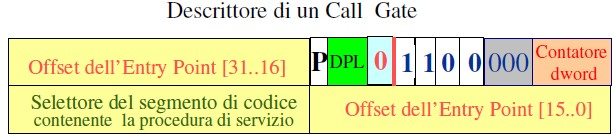
\includegraphics[width=0.65\columnwidth]{img/Callgate}
\caption{Descrittore di un \textit{call gate}}
\label{fig:Callgate}
\end{figure}

Le chiamate a procedura vengono fatte attraverso il \textit{call gate}, che è uno dei famosi "'oggetti di sistema'" noti alla CPU. Anche per i \textit{call gate} esiste un descrittore, in quanto è necessario sapere dove sia l'\textit{entry point} della procedura da chiamare, quali siano i dati per l'accesso, etc\ldots
Perché l'accesso ad una determinata procedura sia valido, si controlla che il livello di privilegio del chiamante sia maggiore o uguale a quello del chiamato. Ad ogni \textit{gate} viene infatti dato un certo livello di privilegio, così come si faceva coi segmenti di dati.

Quando accedo ad una \textit{call gate} (gestita come se fosse un segmento di dati), le istruzioni compiute dalla macchina sono quindi:
\begin{enumerate}
\item si guarda la struttura dalla \textit{call gate} e si prelevano i parametri necessari;
\item si aggiorna il registro CS con l'\textit{entry point};
\item si cambia lo \textit{stack}, sul quale viene salvato anche il puntatore al vecchio \textit{stack};
\item si portano i parametri nello \textit{stack} dedicato alla nostra procedura (tramite un contatore che ci aiuta  a prenderne il giusto numero misurato in \textit{double words}).
\end{enumerate}

\section{\textit{Interrupt gate, trap gate, task gate}}
\label{sec:interruptgate}

Si noti che anche il servizio di un \textit{interrupt}, formalmente, è una chiamata a procedura: nelle macchine Intel, perché esse siano eseguite, viene interpellato l'\textit{interrupt controller} (8254), il quale può gestire fino a 8 \textit{interrupt}.
Nell'8086/88 esiste una \textit{interrupt table} (vedi fig. \ref{fig:interruptTable}), presente all'indirizzo 0 e contenente gli indirizzi per le \textit{routines} di interrupt da servire. Ogni possibile \textit{interrupt} è identificato da 1 byte (per un totale di 256 possibili \textit{interrupt types}) il quale è emesso dal componente 8254 e ci fornisce la giusta chiave per passare alla routine di servizio.

\begin{figure}[!h]
\centering
\includegraphics[width=0.65\columnwidth]{img/interruptTable}
\caption{La \textit{Interrupt table}}
\label{fig:interruptTable}
\end{figure}

\begin{figure}[!h]
\centering
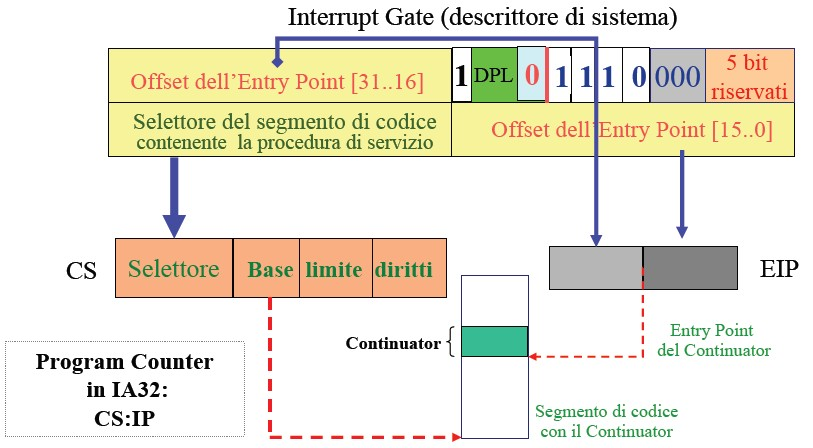
\includegraphics[width=0.75\columnwidth]{img/trasferimentoInterrupt}
\caption{Il meccanismo di trasferimento del controllo alle procedure di servizio dell'\textit{interrupt}}
\label{fig:trasferimentoInterrupt}
\end{figure}

Nell'8086 a partire dall'\textit{interrupt type} eravamo già in grado di ottenere il puntatore alla relativa procedura\footnote{La procedura di servizio dell'\textit{interrupt} farà sempre parte di un segmento di codice, il cui selettore dovrà pertanto essere contenuto nell'\textit{interrupt gate}. La procedura di servizio partirà infatti necessariamente da un certo offset nel suo segmento di codice, il quale dovrà pertanto essere contenuto nell'\textit{interrupt gate}.}. L'\textit{interrupt type} è infatti indice in una tabella che contiene i puntatori agli \textit{entry points} delle procedure di servizio degli \textit{interrupt} (dette anche \textit{continuators}). In un'architettura protetta (IA32) e \textit{multitasking}, invece, dobbiamo dare il puntatore all'\textit{interrupt gate}\footnote{Come distinguiamo un \textit{interrupt gate} da un \textit{task gate}?
\begin{itemize}
\item Se di tipo \textit{interrupt}: identificativo del descrittore = 01110 (E);
\item se di tipo \textit{task}: identificativo del descrittore = 00101 (5).
\end{itemize}
}, descrittore di sistema all'interno dei quali è codificato l'\textit{entry point} della procedura di servizio dell'\textit{interrupt}.

In IA32, queste entità si trovano in una tabella detta \textit{Interrupt Descriptor Table }(IDT, rimpiazzante la tabella IT dell'8086/88) il cui indirizzo lineare iniziale può essere cambiato dal software in quanto viene mantenuto in un apposito registro della CPU detto IDTR.

Quando serviamo un \textit{interrupt}, questi vengono disabilitati e infine riabilitati (IRET) una volta servito il nostro \textit{interrupt}. Se gli \textit{interrupt} sono disabilitati e dobbiamo gestirne degli altri, \emph{annidati}, questo meccanismo non funziona: dobbiamo altresì accoglierli e decidere in base alla priorità degli stessi (esaminata dall'\textit{interrupt controller}). Per questo esiste un modo di servire gli \textit{interrupt}, lasciandoli però abilitati: si fa uso dei \textit{trap gate}.

\begin{figure}[!h]
\centering
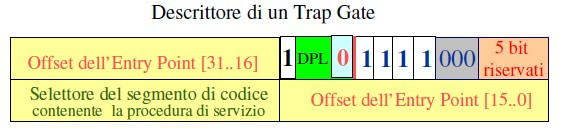
\includegraphics[width=0.65\columnwidth]{img/TrapGate}
\caption{Descrittore del \textit{trap gate}}
\label{fig:TrapGate}
\end{figure}

\begin{figure}[!h]
\centering
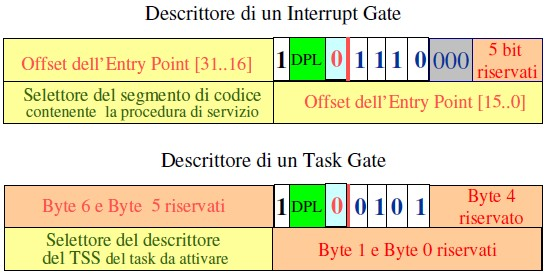
\includegraphics[width=0.65\columnwidth]{img/intTaskGate}
\caption{Descrittore di \textit{task gate} e \textit{interrupt gate}}
\label{fig:intTaskGate}
\end{figure}

La sequenza di procedure nel servire un \textit{interrupt} è quindi la seguente (vedi fig. \ref{fig:percorso}):
\begin{enumerate}
\item arriva un \textit{interrupt};
\item si consulta la IDT;
\item troviamo un \textit{trap gate} relativo alla \textit{routine} di interrupt da gestire;
\item andiamo a pescare il selettore nella GDT;
\item nella GDT sono presenti i descrittori dei TSS di ogni \textit{task};
\item ora che abbiamo il nostro TSS sappiamo quali pagine sono associate al nostro \textit{task} (abbiamo anche i puntatori alla \textit{Page Table} e alla \textit{Page Directory}). Inoltre, abbiamo a disposizione il selettore del descrittore della LDT associata al task;
\item tramite questo selettore accediamo nuovamente alla GDT, dove troviamo il descrittore della LDT;
\item ora finalmente sappiamo dov'è locata la \textit{Local Descriptor Table} e abbiamo così tutto ciò che ci serve per gestire l'\textit{interrupt};
\item finalmente effettuiamo la routine di servizio.
\end{enumerate}

\begin{figure}[!h]
\centering
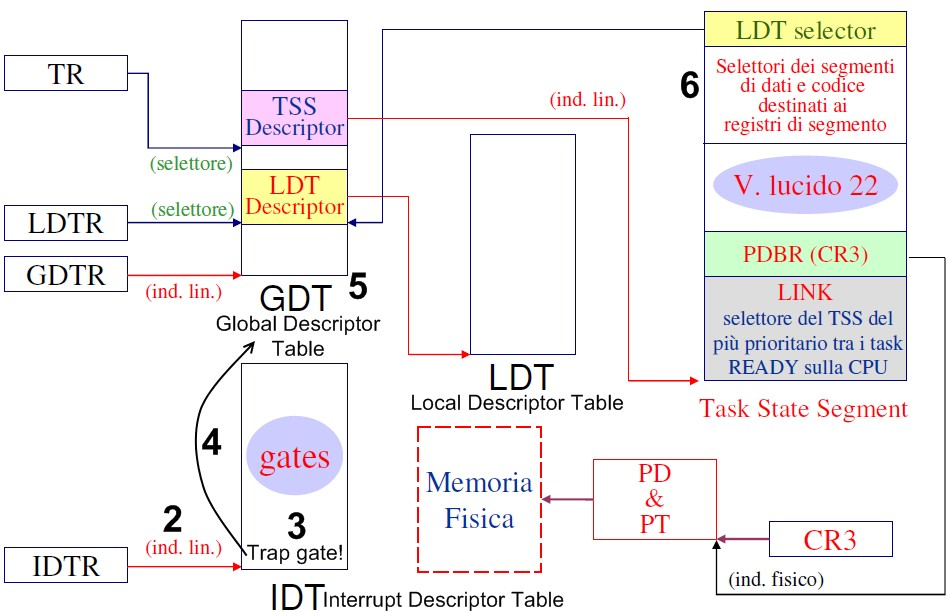
\includegraphics[width=0.93\columnwidth]{img/percorso}
\caption{Percorso di servizio \textit{interrupt}}
\label{fig:percorso}
\end{figure}

\section{\textit{Task call e Task State Segment}}
\label{sec:taskGate}

\begin{figure}[!h]
\centering
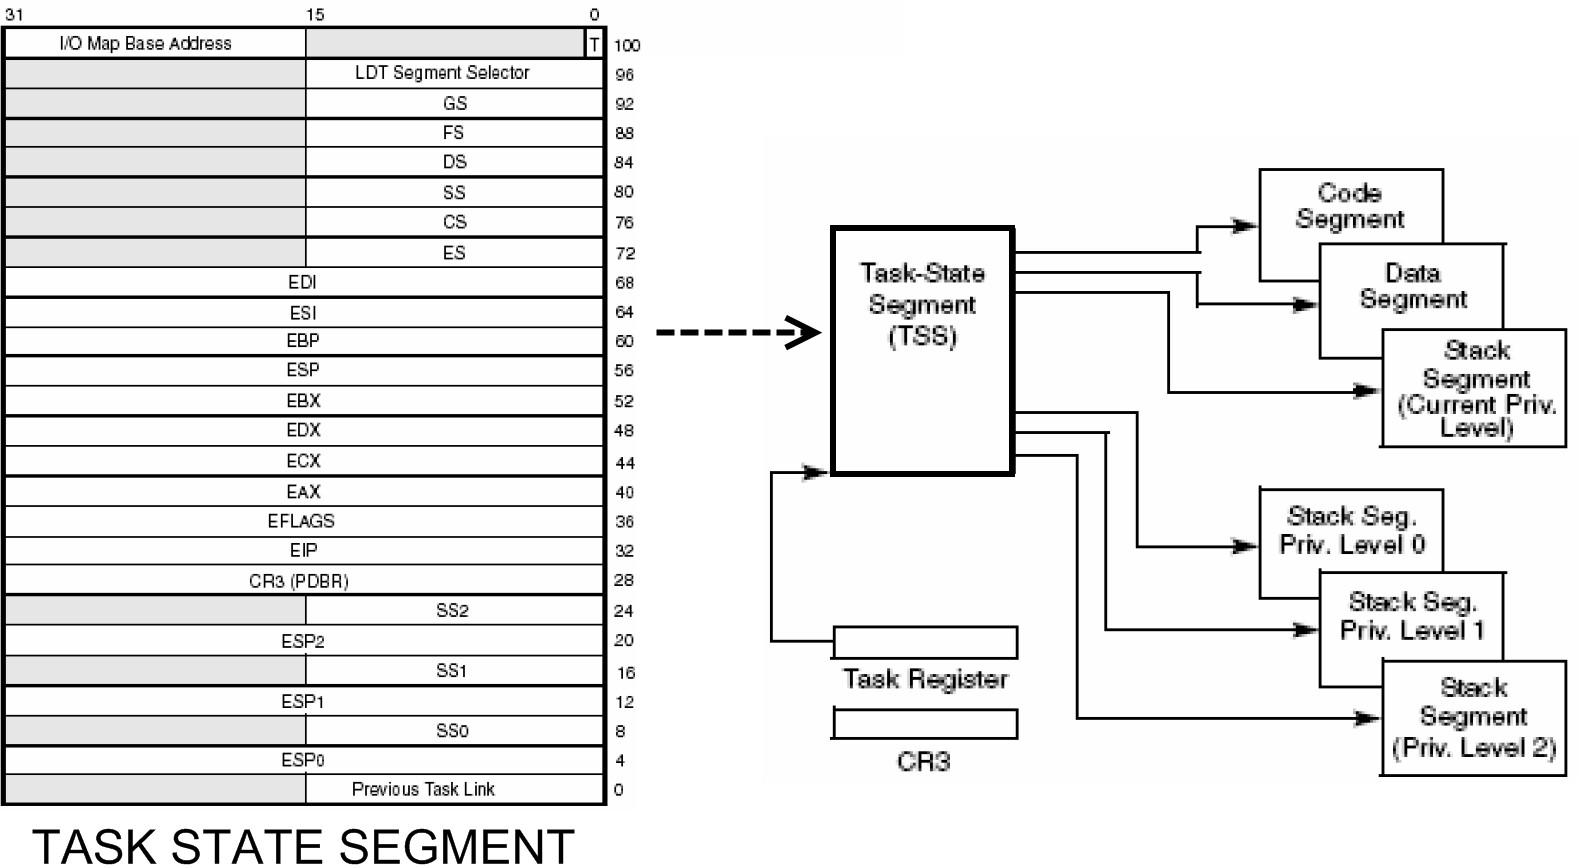
\includegraphics[width=\columnwidth]{img/TSS}
\caption{\textit{Task State Segment}}
\label{fig:TSS}
\end{figure}

Il calcolatore dev'essere naturalmente in grado di gestire molti eventi al secondo, ma ha un unico \textit{program counter} (PC = CS:EIP) il quale dev'essere immediatamente aggiornato nel caso sopraggiungano nuovi elementi da servire: il processo per il quale il processore passa da un compito all'altro è chiamato \textit{context switching} (o \textit{task switching}). Nella nostra macchina possono essere attivi diversi \textit{task}, ognuno con un proprio stato e uno \textit{stack} dove andare a mettere i parametri. Le informazioni riguardanti ogni preciso \textit{task} si trovano nel descrittore del TSS (\textit{Task State Segment}), il quale è un segmento dati con una struttura e dei contenuti ben conosciuti e interpretabili dalla CPU\footnote{Oltre alle informazioni a cui si fa riferimento poco più avanti, il TSS della IA-32 contiene anche le seguenti informazioni
statiche (cioè definite al momento della creazione del task ed eventualmente modificate
dal SO):
\begin{itemize}
\item i selettori dei sei registri di segmento;
\item il valore degli 8 registri di uso generale (EDI, ESI, EBP, ESP, EBX,
EDX, ECX, EAX);
\item il valore del \textit{flag register} EFLAGS;
\item il valore dell'\textit{Instruction Pointer} EIP;
\item il selettore della LDT del \textit{task};
\item il contenuto del registro PDBR col puntatore all'indirizzo fisico della \textit{Page Directory} associata al \textit{task};
\item l'indirizzo logico (selettore e offset) degli \textit{stack} associati al \textit{task} (uno \textit{stack}
per ciascuno dei livelli di privilegio 0, 1 e 2);
\item un bit utilizzato in fase di \textit{debugging};
\item un'area di memoria opzionale a disposizione del sistema operativo(\textit{software state});
\item la mappa dei diritti di accesso alle interfacce di input/output.
\end{itemize}}. Il TSS contiene i riferimenti a codice, dati (registri GS, FS, DS, etc\ldots Essi sono copiati automaticamente nei registri dell'architettura quando si ha l'inizializzazione del \textit{task}) e \textit{stack} di ogni \textit{task}. Tali riferimenti vengono aggiornati ad ogni sospensione e consentono al \textit{task} di ripartire correttamente al momento della successiva messa in esecuzione. Inoltre, come si vede dalla figura \ref{fig:TSS}, il TSS contiene i riferimenti agli \textit{stack} associati ai livelli di privilegio\footnote{Tali riferimenti servono ogni volta che cambia il livello di privilegio del codice in esecuzione (PL decrescente).} da 0 a 2. Infine, il TSS contiene i campi LDT e CR3: il primo è il selettore del descrittore della \textit{Local Descriptor Table} del task, mentre il secondo è il riferimento alle pagine in memoria fisica in cui viene salvata la funzione che trasforma gli indirizzi virtuali del \textit{task} in indirizzi fisici. 
Come dicevamo, ogni TSS ha un descrittore, il quale può risiedere solamente nella GDT.

\begin{figure}[!h]
\centering
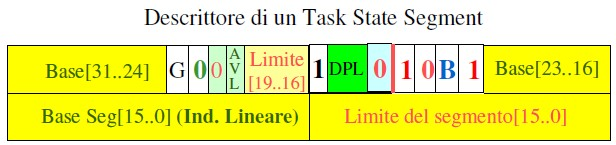
\includegraphics[width=0.65\columnwidth]{img/taskStateSegment}
\caption{Descrittore di un \textit{Task State Segment}}
\label{fig:taskStateSegment}
\end{figure}

In riferimento alla figura \ref{fig:taskStateSegment}, il significato dei campi \textit{Base}, \textit{Limite} e G è analogo a quello dei descrittori di segmenti di codice e dati. Il bit B (\textit{Busy}) vale 1 se il \textit{task} è \textit{running} (cioè in esecuzione) o è \textit{ready} (cioè in attesa di una CPU libera che lo possa mettere in esecuzione); se il bit B vale 0, allora il task è \textit{waiting}, cioè in attesa di un evento che lo attivi (vedi figura \ref{fig:taskStati}). Il tentativo di attivare un \textit{task} che è già attivo (bit B = 1) provoca una eccezione (task non \textit{rientranti}), mentre si può eseguire una seconda istanza di un \textit{task} definendo un secondo \textit{task} associato allo stesso codice. 

\begin{figure}[!h]
\centering
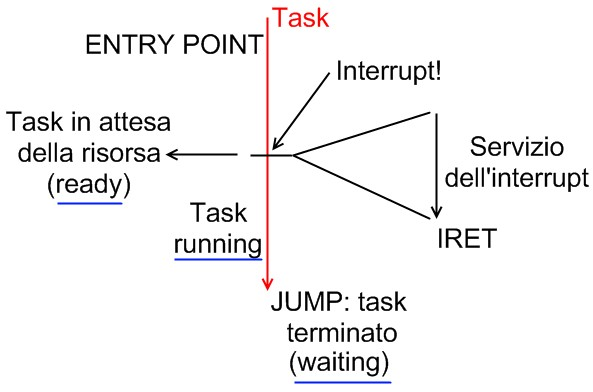
\includegraphics[width=0.55\columnwidth]{img/taskStati}
\caption{Possibili stati di un \textit{task}: \textit{running, ready, waiting}}
\label{fig:taskStati}
\end{figure}

Un \textit{task} può essere attivato non solo in seguito ad un evento, bensì anche in conseguenza della chiamata da parte di un altro \textit{task} (\textit{task call}); alternativamente, si può effettuare una chiamata a \textit{task} simultanea alla terminazione di un altro \textit{task} (istruzione \textit{Jump Task}).
Questo porta alla generazione una catena dinamica in cui ogni \textit{task} punta ad un processo più a valle (cioè a quello che l'ha chiamato), mentre quello più a monte è \textit{running} (vedi fig. \ref{fig:catenaTask}).

\begin{figure}[!h]
\centering
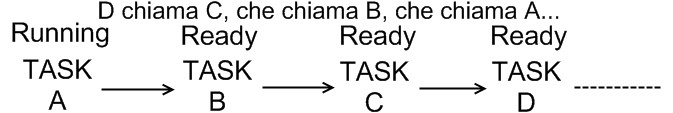
\includegraphics[width=0.65\columnwidth]{img/catenaTask}
\caption{Catena di \textit{task} dinamicamente costruita}
\label{fig:catenaTask}
\end{figure}

Il \textit{Task Register} (TR) è il registro che contiene l'ID del \textit{task} attualmente in \textit{running} (punta al TSS di quest'ultimo): quando un \textit{task} termina o si interrompe e un altro prende il suo posto basta quindi aggiornare il \textit{task register} per effettuare lo scambio. Se ora guardiamo nuovamente il  \textit{task state segment} (figura \ref{fig:TSS}) notiamo la presenza di un campo \textit{link}, puntante al \textit{task} immediatamente più a valle nella catena sopraccitata; se il \textit{task} più a valle della catena ha il campo \textit{link} = 0, non può terminare (non ha nessuno in coda) quindi diventa il \textit{task} IDLE con, come ultima istruzione, HALT.

Si dice anche che i \textit{task} possono essere annidati \textit{nested} (\textit{flag} NT): ovviamente l'ultimo \textit{task}, quello più in coda, ha NT = 0 visto che gli unici \textit{task} in grado di terminare sono quelli più a monte (\textit{nested}).

\begin{figure}[!h]
\centering
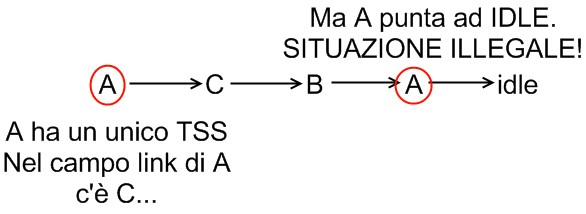
\includegraphics[width=0.59\columnwidth]{img/taskNonRientranti}
\caption{}
\label{fig:taskNonRientranti}
\end{figure}

Ora possiamo meglio capire cosa intendevamo per \textit{task non rientranti}; esaminiamo ad esempio la figura \ref{fig:taskNonRientranti}: la situazione in essa illustrata è illegale in quanto non si può chiamare un \textit{task} che è presente in coda (e, quindi, in stato \textit{ready}). Anche in questo caso il processore riuscirà ad evitare questa eventualità facendo uso del descrittore del TSS.

\section{Sistemi \textit{multiprocessor} e \textit{task}}
\label{sec:multiprocessorTask}

Nel caso di sistemi \textit{multiprocessor} si hanno più \textit{program counter} e, finché ci sono CPU libere, i \textit{task} permangono in \textit{running}. Chiaramente un'architettura così deve poter disporre di una \textit{cache} separata per ogni processore, in modo da sfruttare correttamente il parallelismo: sarebbe demenziale pensare di disporre di più processori ma dover condividere un'unica memoria fisica contendendosi il bus! I processori non potrebbero infatti lavorare contemporaneamente, eventualità auspicabile e che accade davvero nel caso di \textit{cache} separate (una per processore). Il parallelismo sarà tanto più ideale quanto bassa sarà la \textit{miss rate} (ogni tanto saremo costretti ad andare in memoria per forza, facendo uso di un opportuno numero di cicli di bus).

L'architettura del P6 oltre ad essere un'architettura \textit{multitasking} protetta è anche \textit{multiprocessor ready} perché può essere direttamente impiegata nella realizzazione di piattaforme
\textit{multiprocessor} simmetriche UMA (\textit{Uniform Memory Access}). In particolare, la logica di arbitraggio del bus,  i meccanismi di coerenza e i meccanismi di distribuzione delle interruzioni consentono di inserire più CPU in una piattaforma senza apportare altre modifiche e senza bisogno di dover riconfigurare la piattaforma (\textit{multiprocessor ready}).

In generale in una piattaforma multiprocessor IA-32 in ogni istante saranno attive un'unica GDT ed un'unica IDT (i registri GDTR e IDTR di tutte le CPU avranno lo stesso contenuto, vedi paragrafo \ref{sec:tabelleStruttureDati}), mentre ad ogni CPU potrà essere associato un diverso \textit{task} con la sua LDT (pertanto saranno solitamente diversi i contenuti di TR ed LDTR delle diverse CPU, vedi paragrafo \ref{sec:tabelleStruttureDati}).

\section{Tabelle e strutture dati}
\label{sec:tabelleStruttureDati}

Ora che abbiamo introdotto i concetti di descrittore, protezione, privilegi, \textit{task} e \textit{interrupt}, possiamo esaminare con più attenzione le tabelle già introdotte nel paragrafo \ref{sec:descrittori}.

I descrittori dei segmenti di codice e dati e i descrittori degli oggetti di sistema vengono radunati in
tabelle di descrittori organizzate in forma di vettori.
L'architettura IA-32 ha in ogni istante la visibilità dei seguenti 3 vettori di descrittori:
\begin{itemize}
\item  GTD (grandezza massima: 64 KB\footnote{Per un massimo di 8 K descrittori.}; puntata da: GDTR) o \textit{Global Descriptor Table} è una tabella di descrittori accessibili a tutti i \textit{task}. In essa sono contenute tutte le nostre strutture\footnote{E, in particolare,
\begin{itemize}
\item i descrittori dei TSS, e quindi in particolare il TSS \textit{Descriptor} il cui selettore è
caricato in TR (\textit{Task Register});
\item i descrittori dei segmenti di codice e dati comuni a tutti i \textit{task};
\item i descrittori delle LDT di tutti i \textit{task};
\item i descrittori dei \textit{gates} visibili a tutti i \textit{task}.
\end{itemize}};
\item  LDT (puntata da: LDTR) o \textit{Local Descriptor Table} è una tabella di descrittori ridefinita ad ogni operazione di \textit{task switching}; contiene un elenco di descrittori di oggetti (segmenti di codice, descrittori) privati e visibili solo dal \textit{task} a cui la LDT è associata;
\item  IDT (puntata da: IDTR) o \textit{Interrupt Descriptor Table} è una tabella contenente i descrittori dei \textit{gates} di accesso alle procedure o ai \textit{task} associati agli \textit{interrupt}. La IDT corrisponde dunque alla \textit{interrupt table} dell'8086. La IDT può contenere soltanto descrittori di \textit{gate} (\textit{interrupt}, \textit{trap} e \textit{task gate}). L'indice nella IDT è l'\textit{interrupt type}; se a un certo valore di \textit{interrupt type} è associato un \textit{interrupt} o un \textit{trap gate descriptor}\footnote{Ricordiamo che l'unica differenza tra \textit{interrupt gate} e \textit{trap gate} è che quando si mette in servizio una
procedura via \textit{trap gate}, l'\textit{interrupt flag} IF resta a 1 mentre IF viene posto a 0 se si serve
l'eccezione attraverso un \textit{interrupt gate}.}, l'eccezione verrà servita da una semplice procedura mentre, se con \textit{interrupt type} si punta a un \textit{task gate}, il servizio dell'eccezione comporta l'attivazione di un nuovo \textit{task}.
\end{itemize}

\begin{figure}[!h]
\centering
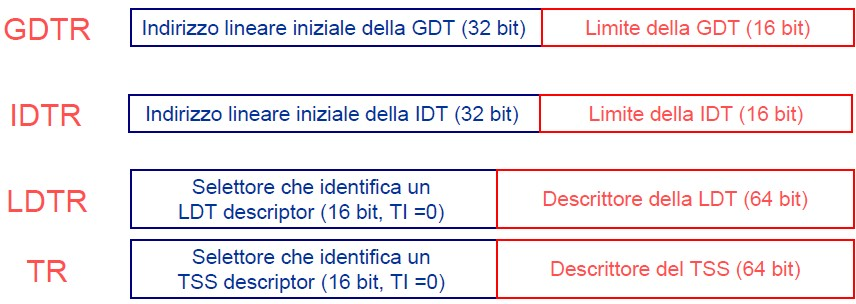
\includegraphics[width=0.75\columnwidth]{img/selettori}
\caption{Struttura dei registri che puntano le varie tabelle}
\label{fig:selettori}
\end{figure}

In figura \ref{fig:selettori} viene riportata la struttura dei selettori per le varie tabelle:
Il formato dei registri GDTR e IDTR è detto \textit{pseudo descriptor} perché contiene un sottoinsieme dei campi inclusi in un descrittore. Il campo \textit{limite} consente alla CPU di verificare la legittimità del selettore (un indice che punta oltre il limite della tabella provoca una eccezione di violazione della protezione).

In LDTR e TR solo i 16 bit con il selettore sono visibili al software (cioè al linguaggio macchina); i 64 bit col descrittore sono una copia del descrittore presente in GDT. Il descrittore viene automaticamente caricato nel registro per consentire alla CPU di gestire la protezione sul TSS e sulla LDT senza aver bisogno di accedere ala
memoria (ove risiede la GDT). LDTR e TR vengono aggiornati automaticamente ad ogni operazione di \textit{task switching}, ma esistono anche istruzioni specifiche in linguaggio macchina per aggiornarli e leggerli.




